\documentclass[12pt]{article}
\usepackage[margin=1in, headheight=20pt]{geometry}
\usepackage{xcolor}
\usepackage{tikz}
\usepackage{pgfplots}
\usepackage{eso-pic}
\usepackage{amsmath, amsthm, amssymb}
\usepackage{mathtools}
\usepackage[italicdiff]{physics}
\usepackage{enumitem}
\usepackage{lmodern}
\usepackage{fancyhdr}
\usepackage{pgfornament}
\usepackage{parskip}

\definecolor{pagecolor}{HTML}{DCE2F0}
\definecolor{textcolor}{HTML}{373D4A}

\definecolor{quasicolor}{HTML}{5E4E9C}
\definecolor{taxicabcolor}{HTML}{4169B0}
\definecolor{euclideancolor}{HTML}{0080C4}
\definecolor{infinitycolor}{HTML}{009EE3}

\pagecolor{pagecolor}
\color{textcolor}

\AddToShipoutPictureBG{
  
\begin{tikzpicture}[remember picture, overlay]
    \draw[
      line width=0.5pt,
      color=textcolor,
      opacity=0.075
    ]
    (current page.south west) grid[step=10pt] (current page.north east);
  \end{tikzpicture}
}

\pagestyle{fancy}
\fancyhf{}
\fancyhead[L]{Numerical Optimization}
\fancyhead[R]{\nouppercase{\leftmark}}
\fancyfoot[C]{}

\renewcommand{\headrule}{
  \vspace{-5pt}
  \hbox to \headwidth{
    \leaders\hrule height 0.5pt\hfill
    \hspace{5pt}
    \raisebox{0.20pt}{\pgfornament[width=1cm]{11}}
    \hspace{5pt}
    \leaders\hrule height 0.5pt\hfill
  }
}

\renewcommand{\footrule}{
  \vspace{-12pt}
  \hbox to \headwidth{
    \leaders\hrule height 3.5pt depth -3pt \hfill 
    \hspace{5pt} 
    \thepage 
    \hspace{5pt}
    \leaders\hrule height 3.5pt depth -3pt \hfill
  }
}

\fancypagestyle{plain}{
  \fancyhf{}
  \renewcommand{\headrulewidth}{0pt}
  \renewcommand{\headrule}{} 
  \fancyfoot[C]{}
  \renewcommand{\footrule}{
    \vspace{-12pt}
    \hbox to \headwidth{
      \rule[0.65ex]{0.47\headwidth}{0.5pt}%
      \hfill
      \thepage
      \hfill
      \rule[0.65ex]{0.47\headwidth}{0.5pt}%
    }
  }
}

\newcommand{\ds}{\displaystyle}

\newcommand{\bb}[1]{\mathbb{#1}}
\newcommand{\cl}[1]{\mathcal{#1}}

\newcommand{\p}[1]{\left ( #1 \right )}
\newcommand{\bk}[1]{\left [ #1 \right ]}
\newcommand{\br}[1]{\left \{ #1 \}}
\newcommand{\ab}[1]{\langle #1 \rangle}

\newcommand{\f}[2]{\frac{#1}{#2}}
\newcommand{\nset}{\varnothing}
\newcommand{\oo}{\infty}

\newcommand{\gm}{\gamma}
\newcommand{\de}{\delta}
\newcommand{\De}{\Delta}
\newcommand{\ep}{\varepsilon}
\newcommand{\la}{\lambda}
\newcommand{\si}{\sigma}
\newcommand{\om}{\omega}
\newcommand{\Om}{\Omega}

\newcommand{\imp}{\Rightarrow}
\newcommand{\pmi}{\Leftarrow}
\renewcommand{\iff}{\Leftrightarrow}
\newcommand{\ffi}{\Rightarrow\!\Leftarrow}

\setlist[enumerate]{label=(\alph*)}
\pgfplotsset{compat=newest}

\newtheoremstyle{boldnote}
  {}
  {}
  {\itshape}
  {}
  {\bfseries}
  {.}
  { }
  {\thmname{#1}\thmnumber{ #2}\thmnote{ (\bfseries #3)}}
\theoremstyle{boldnote}
\newtheorem{theorem}{Theorem}[section]
\newtheorem{lemma}[theorem]{Lemma}

\theoremstyle{definition}
\newtheorem{definition}[theorem]{Definition}
\newtheorem{example}{Example}

\title{
    \textbf{Numerical Optimization} \\
}
\author{
    Dhyan Laad \\
    \texttt{2024ADPS0875G}
}
\date{}

\begin{document}
\maketitle
\tableofcontents
\newpage

\section{Preliminaries}
\subsection{Inner Product Spaces}
\begin{definition}
    Let $V$ be a real vector space. A function $\ab{\cdot, \cdot} : V \times V \to \bb R$ is called a \emph{real inner product} if it satisfies the following properties for $x, y, z \in V$ and $c \in \bb R$:
    \begin{enumerate}
        \item $\ab{x, y} = \ab{y, x}$,
        \item $\ab{x + z, y} = \ab{x, y} + \ab{z, y}$,
        \item $\ab{cx, y} = c\ab{x, y}$, and
        \item $\ab{x, x} \geq 0$ and $\ab{x, x} = 0 \iff x = 0$.
    \end{enumerate}
\end{definition}

The inner product is the generalization of the dot product on Euclidean vector spaces: for $\vb x = (x_1, x_2, \dots , x_n)$ and $\vb y = (y_1, y_2, \dots , y_n)$ where $x_i, y_i \in \bb R$ for $i \in 1 : n$,
\[\vb x \cdot \vb y = \sum_{i=1}^n x_iy_i.\]
It may also be defined on $\bb C$-spaces, replacing (a) with conjugate symmetry: $\ab{x, y} = \overline{\ab{y, x}}$, and adding conjugate linearity in the second argument: $\ab{x, cy} = \bar{c}\ab{x, y}$.

\begin{definition}
    Let $V$ be a real vector space and $\ab{\cdot, \cdot}$ an inner product. Then, $(V, \ab{\cdot, \cdot})$ is called a \emph{real inner product space}.
\end{definition}

For brevity, we may simply state that $V$ is an inner product space, with the notation for the inner product being implicit, and all future inner product spaces map into $\bb R$ unless stated otherwise.

\subsection{Normed Linear Spaces}
\begin{definition}
    Let $V$ be a real vector space. A function $\norm{\cdot} : V \to \bb R$ is called a \emph{norm} if it satisfies the following properties for $x, y \in V$ and $c \in \bb R$:
    \begin{enumerate}
        \item $\norm{cx} = \abs{c} \norm{x}$,
        \item $\norm{x} \geq 0$ and $\norm{x} = 0 \iff x = 0$, and
        \item $\norm{x + y} \leq \norm{x} + \norm{y}$.
    \end{enumerate}
\end{definition}

This last property is referred to as the \emph{triangle inequality}. The norm assigns a notion of length to vectors, and generalizes the standard formula for the length of a vector in a Euclidean vector space: for $\vb x = (x_1, x_2, \dots , x_n)^\top$ where $x_i \in \bb R$ for $i \in 1 : n$.
\[\norm{\vb x} = \p{\sum_{i=1}^n x_i^2}^{1/2}.\]

\begin{definition}
    Let $V$ be a vector space and $\norm{\cdot}$ a norm. Then $(V, \norm{\cdot})$ is called a \emph{normed linear space}.
\end{definition}

Once again, we may conventionally omit the norm from notation when defining a new normed linear space.

\begin{definition}
    Let $p \geq 1$. The \emph{$p$-norm} (or \emph{$\ell^p$-norm}) of a vector $\vb x = (x_1, x_2, \dots, x_n)^\top$ where $x_i \in \bb R$ for $i \in 1 : n$ is
    \[\norm{\vb x}_p \coloneqq \p{\sum_{i=1}^n \abs{x_i}^p}^{1/p}.\]

    For $p=1$, we get the \emph{taxicab} or \emph{Manhattan} norm, for $p=2$, we get the standard Euclidean norm, and for $p \to \oo$, the $p$-norm approaches the \emph{infinity} or \emph{maximum} norm:
    \[\norm{\vb x}_\oo \coloneqq \max_{i} \abs{x_i}.\]
\end{definition}

For $p \in (0, 1)$, the triangle inequality does not hold, and the resulting functions are called \emph{quasinorms}. Pictured below are unit circles in the $0.5$-quasinorm, and $p$-norms for $p \in \{1, 2, \oo\}$.

\begin{center}
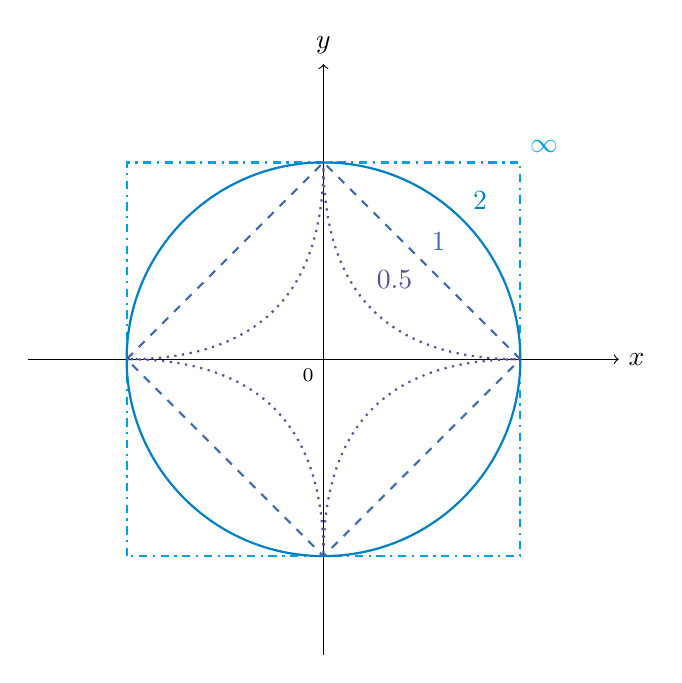
\begin{tikzpicture}[scale=2.5]

    % Axes
    \draw[->] (-1.5,0) -- (1.5,0) node[right] {$x$};
    \draw[->] (0,-1.5) -- (0,1.5) node[above] {$y$};
    \node[below left, font=\scriptsize] at (0,0) {0};

    % Infinity norm
    \draw[infinitycolor, thick, dashdotted] (-1,-1) rectangle (1,1);
    \node[infinitycolor, above right] at (1,1) {$\oo$};

    % Euclidean norm
    \draw[euclideancolor, thick] (0,0) circle (1cm);
    \node[euclideancolor, above right] at (0.71, 0.71) {2};

    % Taxicab norm
    \draw[taxicabcolor, thick, dashed] (1,0) -- (0,1) -- (-1,0) -- (0,-1) -- cycle;
    \node[taxicabcolor, right] at (0.5, 0.6) {1};

    % Quasinorm (1/2)
    \draw[quasicolor, thick, dotted] 
        plot[domain=0:360, samples=200, smooth] 
        ({sign(cos(\x))*abs(cos(\x))^4}, {sign(sin(\x))*abs(sin(\x))^4});
    \node[quasicolor, below left] at (0.5, 0.5) {$0.5$};

\end{tikzpicture}
\end{center}

\begin{lemma}
  Let $V$ be a normed linear space. Then,
  \[\abs{\norm{x} - \norm{y}} \leq \norm{x - y}\]
  for every $x, y \in V$.
\end{lemma}

\begin{theorem}
  Let $(V, \norm{\cdot})$ be a normed linear space. Then $\norm{\cdot} : V \to \bb R$ is uniformly continuous.
\end{theorem}
\begin{proof}
  Let $\ep > 0$, and choose $\de = \ep$. If $\norm{x - y} < \de$, then by Lemma 1.6,
  \[\abs{\norm{x} - \norm{y}} \leq \norm{x - y} < \de = \ep.\]
  Therefore, $\abs{\norm{x} - \norm{y}} < \ep$.
\end{proof}

\begin{theorem}
  Every inner product space $V$ is naturally a normed linear space. For $x \in V$ define
  \[\norm{x} \coloneqq \sqrt{\ab{x, x}}.\]
\end{theorem}

However, the converse is not always true.

\begin{theorem}
  A normed linear space $V$ is an inner product space iff the norm satisfies the parallelogram law:
  \[\norm{x + y}^2 + \norm{x - y}^2 = 2(\norm{x}^2 + \norm{y}^2).\]
  The inner product is given by
  \[\ab{x, y} = \f 14 \p{\norm{x + y}^2 - \norm{x - y}^2}\]
  for all $x, y \in V$.
\end{theorem}

We now look at a fundamental theorem in linear algebra.
\begin{theorem}[Cauchy-Schwarz Inequality]
  Let $V$ be an inner product space with an induced norm. Then for all $x, y \in V$
  \[\abs{\ab{x, y}} \leq \norm{x}\norm{y}.\]
\end{theorem}
\begin{proof}
  We utilize the discriminant of a quadratic equation and the nonnegativity of the norm. Firstly, if $y = 0$, then the inequality holds trivially. For $y \neq 0$, consider the vector $x + ty$ for some $t \in \bb R$. Then
  \[0 \leq \norm{x + ty}^2 = \ab{x+ty, x+ty} = \norm{y}^2t^2 + 2\ab{x, y}t + \norm{x}^2.\]
  Since the quadratic in $t$ is nonnegative, its discriminant must be nonpositive, giving us
  \[4\ab{x, y}^2 - 4\norm{x}^2\norm{y}^2 \leq 0 \imp \abs{\ab{x, y}} \leq \norm{x}\norm{y}.\]
\end{proof}

\subsection{Eigenvalues and Eigenvectors}
\begin{definition}
  Let $A$ be a square matrix of order $n$. Then, $\la$ is said to be an \emph{eigenvalue} of $A$ if there exists nonzero $\vb x \in \bb R^n$ such that
  \[A\vb x = \la \vb x.\]
  Here, $\vb x$ is called an \emph{eigenvector} corresponding to $\la$.
\end{definition}

To find the eigenvalues of an arbitrary matrix, consider the following:
\[A\vb x = \la \vb x \imp A\vb x - \la \vb x = \vb 0 \imp (A - \la I)\vb x = \vb 0.\]
Since $\vb x$ is nonzero, we require the matrix $A - \la I$ to be singular. That is,
\[\det(A - \la I) = 0.\]
The left side of the equation is a polynomial in $\la$, and is called the \emph{characteristic polynomial}. Therefore the eigenvalues of a matrix $A$ are the \emph{roots} to its characteristic polynomial.

\begin{theorem}
  Eigenvectors corresponding to distinct eigenvalues are linearly independent.
\end{theorem}

\begin{definition}
  A square matrix $A$ is said to be diagonalizable if there exists an invertible matrix $P$ such that
  \[P^{-1}AP = D\]
  where $D$ is a diagonal matrix.
\end{definition}

It turns out that in Definition 1.13, the entries of $D$ along the diagonal are the eigenvalues of $A$, and $P$ contains corresponding eigenvectors in the respective columns of the eigenvalues in $D$.

\subsection{Quadratic Forms}
Certain quadratic functions of several variables may be represented using matrices.
\begin{definition}
  A \emph{quadratic form} is a homogenous polynomial of degree $2$ in multiple variables.
\end{definition}

A quadratic form in $n$ variables may be written with a symmetric matrix $A$ of order $n$ and a vector $\vb x = (x_1, x_2, \dots, x_n)^\top$ of unknowns:
\[Q(x) = \ab{A\vb x, \vb x} = \vb x^\top A\vb x = \sum_{i=1}^n a_{ii}x_{i}^2 + \underset{i \neq j}{\sum_{i=1}^n\sum_{j=1}^n} a_{ij}x_ix_j\]
where $a_{ij}$ is the $(i,j)$th entry of $A$.

\begin{definition}
  Let $A$ be a square matrix of order $n$, and let $p = \ab{A\vb x, \vb x}$. If for all nonzero $\vb x \in \bb R^n$
  \begin{enumerate}
    \item $p > 0$, then $A$ is said to be \emph{positive definite},
    \item $p \geq 0$, \emph{positive semidefinite},
    \item $p < 0$, \emph{negative definite}, and
    \item $p \leq 0$, \emph{negative semidefinite}.
  \end{enumerate}
  Otherwise, $A$ is said to be \emph{indefinite}.
\end{definition}

The definiteness of a matrix may also be realized through its principal minors.

\begin{definition}
  Let $A$ be a square matrix of size $n$. A \emph{principal minor of order $k$} of $A$ may be computed by the following.
  \begin{enumerate}[label=\arabic*.]
    \item Choose any set of $k$ indices $\{i_1, i_2, \dots, i_k\}$ from $\{1, 2, \dots , n\}$.
    \item Keep the rows and columns corresponding to these indices, creating a $k \times k$ submatrix.
    \item Take the determinant of this resulting submatrix to yield a principal minor of order $k$.
  \end{enumerate}
  If the first $k$ indices $\{1, 2, \dots, k\}$ are chosen, then the resulting principal minors called \emph{leading principal minors of order $k$}.
\end{definition}

\begin{theorem}
  A square matrix is
  \begin{enumerate}[font=\upshape]
    \item positive definite iff all leading principle minors are positive,
    \item positive semidefinite iff all principal minors are nonnegative,
    \item negative definite iff the $k$th leading principal minor has the sign of $(-1)^k$, and
    \item negative semidefinite iff all principal minors of order $k$ either have the sign of $(-1)^k$ or are $0$.
  \end{enumerate}
  A matrix that does not fall into the aforementioned categories is indefinite.
\end{theorem}

We may also characterize definiteness using a matrix's eigenvalues.
\begin{theorem}
  A square matrix of order $n$ with eigenvalues $\la_i$ for $i \in 1 : n$ is
  \begin{enumerate}[font=\upshape]
    \item positive definite iff $\la_i > 0$ for all $i$,
    \item positive semidefinite iff $\la_i \geq 0$ for all $i$,
    \item negative definite iff $\la_i < 0$ for all $i$, and
    \item negative semidefinite iff $\la_i \leq 0$ for all $i$.
  \end{enumerate}
  A matrix that does not fall into the aforementioned categories is indefinite.
\end{theorem}

\subsection{Matrix Norms}
\begin{definition}
  Let $\bb R^{m \times n}$ denote the set of all matrices of size $m \times n$ with real entries. A function $\norm{\cdot} : \bb R^{m \times n} \to \bb R$ is called a \emph{real matrix norm} if it satisfies the following properties for $c \in \bb R$ and $A, B \in \bb R^{m \times n}$:
  \begin{enumerate}
    \item $\norm{A} \geq 0$ and $\norm{A} = 0 \iff A = \vb 0$,
    \item $\norm{cA} = \abs{c}\norm{A}$,
    \item $\norm{A + B} \leq \norm{A} + \norm{B}$, and
    \item $\norm{AB} \leq \norm{A}\norm{B}$ for $m = n$.
  \end{enumerate}
\end{definition}

Four of the most widely used ones are detailed below for a square matrix $A = [a_{ij}]_n$.
\begin{description}
  \item[$\boldsymbol{1}$-norm.] The $1$-norm is the \emph{maximum absolute column sum}:
  \[\norm{A}_1 = \max_{1 \leq j \leq n} \sum_{i=1}^n \abs{a_{ij}}.\]
  \item[$\boldsymbol{\oo}$-norm.] The $\oo$-norm is the \emph{maximum absolute row sum}:
  \[\norm{A}_\oo = \max_{1 \leq i \leq n} \sum_{j=1}^n \abs{a_{ij}}.\]
  \item[$\boldsymbol{2}$-norm.] The $2$-norm is also called the \emph{spectral norm} and is given by
  \[\norm{A}_2 = \sqrt{\la_{\mathrm{max}}(A^\top A)}\]
  where $\la_\mathrm{max}(M)$ is the largest eigenvalue of $M$.
  \item[Frobenius norm.] The Frobenius norm is the sum of the squared entries of the matrix:
  \[\norm{A}_F = \p{\sum_{i=1}^n\sum_{j=1}^n a_{ij}^2}^{1/2} = \sqrt{\tr(A^\top A)}\]
  where $\tr(M)$ is the trace of $M$.
\end{description}

In general, a specific matrix norm can be induced from an existing vector norm by defining
\[\norm{A} = \sup_{\vb x \neq 0} \f{\norm{A\vb x}}{\norm{\vb x}}.\]

\section{Calculus}

\subsection{Extreme Points}
We start by reviewing and defining the concepts of a minimum and maximum from elementary calculus. Let $I = [a, b] \subset \bb R$ and $f : I \to \bb R$.

\begin{definition}
  $x^* \in I$ is said to be a \emph{local minimum} of $f$ if there exists $\de > 0$ such that $f(x^*) \leq f(x)$ for all $x \in B(x^*, \de)$.
\end{definition}

\begin{definition}
  $x^* \in I$ is said to be a \emph{local maximum} of $f$ if there exists $\de > 0$ such that $f(x^*) \geq f(x)$ for all $x \in B(x^*, \de)$.
\end{definition}

\begin{definition}
  $x^* \in I$ is said to be a \emph{global minimum} of $f$ if $f(x^*) \leq f(x)$ for all $x \in I$.
\end{definition}

\begin{definition}
  $x^* \in I$ is said to be a \emph{global maximum} of $f$ if $f(x^*) \geq f(x)$ for all $x \in I$.
\end{definition}

The definitions for the corresponding strict versions of the maxima and minima may be obtained by simply replacing the inequality with a strict one. The point $x^*$ is called a \emph{minimizer} of \emph{maximizer}.

\begin{theorem}
  Let $x^*$ be a local minimizer of $f$ and let $x^*$ be an interior point of $I = [a, b]$. If $f$ is differentiable at $x^*$, then $f'(x^*) = 0$.
\end{theorem}
\begin{proof}
  Since $x^*$ is a local minimizer and an interior point of $I$, there exists $\de > 0$ such that $f(x^*) \leq f(x)$ for all $x \in B(x^*, \de)$. For $h > 0$ such that $h < \de$,
  \[f(x^*) \leq f(x^* + h) \quad \text{and} \quad f(x^*) \leq f(x^* + h). \]
  We know that $f$ is differentiable at $x^*$. As such,
  \begin{align*}
    f'(x^*) &= f_+'(x^*) = \lim_{h \to 0^+} \f{f(x^* + h) - f(x^*)}{h}, \\
    f'(x^*) &= f_-'(x^*) = \lim_{h \to 0^+} \f{f(x^*) - f(x^* - h)}{h}.
  \end{align*}
  As such, $f'(x^*) = f_+'(x^*) \geq 0$ and $f'(x^*) = f_-'(x^*) \leq 0$, and therefore $f'(x^*) = 0$.
\end{proof}

An analogous result holds for a maximizer.
\begin{theorem}
  Let $x^*$ be a local maximizer of $f$ and let $x^*$ be an interior point of $I = [a, b]$. If $f$ is differentiable at $x^*$, then $f'(x^*) = 0$.
\end{theorem}

\begin{definition}
  Let $f : [a, b] \to \bb R$, and $x^* \in (a, b)$. If $f$ is differentiable at $x^*$ and $f'(x^*) = 0$, or if $f$ is not differentiable at $x^*$, it is said to be a \emph{critical point of $f$}.
\end{definition}

\begin{definition}
  Let $f : [a, b] \to \bb R$, and $x^* \in (a, b)$. If $f$ is differentiable at $x^*$ and $f'(x^*) = 0$, then it is said to be a \emph{stationary point of $f$}.
\end{definition}

We now proceed to list out a few preliminary results of use.

\begin{theorem}[Weierstrass Extreme Value Theorem]
  Let $S$ be a compact set, and $f : S \to \bb R$ be a continuous mapping. Then, $f$ attains a global maximum and a global minimum on $S$.
\end{theorem}

\begin{theorem}[Closed Point Theorem]
  Let $S$ be a nonempty, closed, and convex set in $\bb R^n$, and $y \not \in S$. Then, there exists a unique point $x^* \in S$ such that
  \[\norm{y - x^*} \leq \norm{y - x} \]
  for all $x \in S$. Thus, $x^*$ is the minimizing point iff
  \[(y - x^*)^\top(x - x^*) \leq 0\]
  for all $x \in S$.
\end{theorem}

\begin{theorem}[Taylor's Theorem]
  Let $I \subseteq \bb R$ be an interval, $f : I \to \bb R$ such that $f \in \cl C^n(I)$, and $x, x^* \in I$. Let $h = x - x^*$. Then, there exists $\xi \in (0, 1)$ such that
  \[f(x) = f(x^*) + hf^{(1)}(x^*) + \f{h^2}{2!}f^{(2)}(x^*) + \cdots + \f{h^{n-1}}{(n-1)!}f^{(n-1)}(x^*) + \f{h^n}{n!}f^{(n)}(x^* + \xi h).\]
\end{theorem}

The proofs of the above theorems have been omitted for brevity.

\begin{theorem}
  Let $I \subseteq \bb R$ be an interval, $f \in \cl C^2(I)$, and $x^*$ a critical point of $f$.
  \begin{enumerate}[font=\upshape]
    \item If $f^{(2)}(x^*) > 0$ for all $x \in I$, then $x^*$ is a global minimizer of $f$.
    \item If $f^{(2)}(x^*) < 0$, for all $x \in I$, then $x^*$ is a global maximizer of $f$.
  \end{enumerate}
\end{theorem}
\begin{proof}
  Let $x \in I$ and $h = x - x^*$. By Taylor's Theorem,
  \[f(x) = f(x^*) + hf^{(1)}(x^*) + \f{h^2}{2}f^{(2)}(x^* + \xi h)\]
  for some $\xi \in (0, 1)$. Since $x^*$ is a critical point of $f$, $f^{(1)}(x^*) = 0$. Therefore,
  \[f(x) - f(x^*) = \f{h^2}{2}f^{(2)}(x^* + \xi h).\]
  If $f^{(2)}(x) > 0$ for all $x \in I$, then $f(x) - f(x^*) > 0$ for all $x \neq x^*$, and thus $x^*$ is a global minimizer of $f$. Similarly, if $f^{(2)}(x) < 0$ for all $x \in I$, then $f(x) - f(x^*) < 0$ for all $x \neq x^*$, and thus $x^*$ is a global maximizer of $f$.
\end{proof}

\subsection{Multivariable Calculus}
We first explore differentiability of multivariable functions.
\begin{definition}
  Let $\Om \subseteq \bb R^n$. A function $f : \Om \to \bb R$ is said to be \emph{differentiable at $x^* \in \Om$} if the partial derivatives
  \[f_{x_i} \equiv \pdv{f}{x_i}, \quad i \in \{1, 2, \dots, n\},\]
  exist. Furthermore, the \emph{gradient} of $f$ at $x^*$ is defined as
  \[\nabla f(x^*) \coloneqq \bk{\pdv{f}{x_1}(x^*) \; \pdv{f}{x_2}(x^*) \; \dots \; \pdv{f}{x_n}(x^*)}^\top.\]
\end{definition}

\begin{definition}
  Let $\Om \subseteq \bb R^n$. The \emph{Hessian} of a function $f : \Om \to \bb R$ at $x^* \in \Om$ is defined as the square matrix of second-order partial derivatives:
  \[H_f(x^*) =
  \begin{bmatrix}
    f_{x_1 x_1}(x^*) & f_{x_1 x_2}(x^*) & \dots & f_{x_1 x_n}(x^*) \\
    f_{x_2 x_1}(x^*) & f_{x_2 x_2}(x^*) & \dots & f_{x_2 x_n}(x^*) \\
    \vdots & \vdots & \ddots & \vdots \\
    f_{x_n x_1}(x^*) & f_{x_n x_2}(x^*) & \dots & f_{x_n x_n}(x^*)
  \end{bmatrix}.
  \]
\end{definition}
If the function $f$ is continuously differentiable at $x^*$, then the Hessian is symmetric.

\begin{definition}
  A vector valued function $f : [a, b] \to \bb R^n$ is said to be \emph{differentiable at $x^* \in [a, b]$} if all of its component functions $f_i : [a, b] \to \bb R$ for $i \in 1 : n$ are differentiable at $x^*$.
  \[f'(x^*) = \bk{f'_1(x^*) \; f'_2(x^*) \; \cdots \; f'_n(x^*)}^\top\]
\end{definition}

Now consider two functions:
\begin{itemize}
  \item $f : \Om \to [a, b]$, where $\Om \subseteq \bb R$.
  \item $g : [a, b] \to \Om$.
\end{itemize}
We are interested in the differentiability of the composition $h = f \circ g : [a, b] \to [a, b]$. The derivative is given by the chain rule:
\[h'(t) = \nabla f(g(t))g'(t).\]

We may also extend the notion of Taylor series to multivariable functions. For a smooth function $f : \bb R^2 \to \bb R$,
\[f(x + h, y + h) = \sum_{k=0}^\oo \f{(h\partial_x + k\partial_y)^k}{k!} f(x, y).\]

\begin{definition}
  The \emph{level set} of a function $f : \Om \to \bb R$ at $c \in \bb R$ is defined as
  \[L_c = \{x \in \Om : f(x) = c\}.\]
\end{definition}
\end{document}